\documentclass[9pt,twocolumn,twoside]{styles/osajnl}
\usepackage{fancyvrb}
\journal{i524} 
%\usepackage[nomarkers,figuresonly]{endfloat}

\title{\centering%
Nagios (Example Paper for I524)}


\author[1]{Tony Liu}
\author[1]{Vibhatha Abeykoon}
\author[1]{Gregor von Laszewski}


\affil[1]{School of Informatics and Computing, Bloomington, IN 47408, U.S.A.}


\dates{status: early draft, paper-1, HID ???, HID ???, HID ???\today}

\ociscodes{Cloud, I524}

% replace this with your url in github/gitlab
\doi{\url{https://github.com/vibhatha/sp17-i524/blob/master/paper1/S17-TS-0003/report.pdf}}


\begin{abstract} Nagios is a system, network and infrastructure
  monitoring tool providing instant awareness of IT infrastructure.
  Nagios allows to monitor the infrastructure, alert the system admin,
  provide visualized reports, schedule downtime for maintenance, and
  plan upgrade in advance with trends and capacity diagrams. The
  design emphasizes highly on flexibility and scalability. We
  summarize details of Nagios and outline how it is useful as part
  ofthe services used in big data. \end{abstract}

\setboolean{displaycopyright}{true}

\begin{document}

\maketitle

\section{Introduction}

Nagios ~\cite{www-nagios, wiki-nagios} is a system, network and
infrastructure monitoring tool under open source license that provides
instant awareness of mission-critical IT infrastructure. Nagios allows
to monitor the infrastructure, alert the system admin, provide
visualized reports, schedule downtime for maintenance, and plan
upgrade in advance with trends and capacity diagrams. Its design
emphasizes highly on flexibility and scalability. To provide such
flexibility, Nagios is composed of different modules. Through the
modular design Nagios cab adapts easily to systems and networks
monitoring needed by different users. It also allows integration of new
components that allow adaptation towards service monitoring needs that
have not yet been distributed with Nagios, allowing extensibility.

\subsection{Architecture}

Nagios \cite{nagios-paper-2012} flexible modular architecture allows
users to customize modules to monitor the network and
infrastructure. We show the elementary Nagios archirtecture in
Figure~\ref{fig:Nagios-architecture} ~\cite{nagios-book}.

\begin{figure}[htb]
\centering
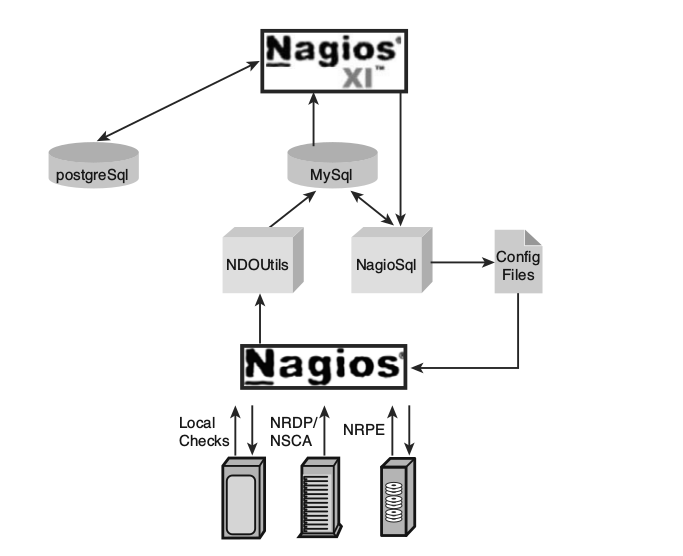
\includegraphics[width=\columnwidth]{images/nagios-architecture}
\caption{Nagios Architecture~\cite{nagios-book}.}
\label{fig:Nagios-architecture}
\end{figure}

Nagios architecture consists of two main databases. They are MySQL and
Postgre SQL.  Nagios XI is directly connected with MySQL and Postgre
SQL. There are two main components connected with MySQL, NDOUtils and
NagioSQL are these two components. The NagiosSQL refers to the
configuration files to get configuration parameters. Nagios local
installation is also connected with three main components. They are
Local Checks, NRDP/NSCA and NRPE components.

Nagios has a number of components such as Nagios core, file system,
Nagios daemon, services, plugins, event handlers, performance processors
and notification commands.

The main component is {\em Nagios core}, which is a scheduler daemon
detecting network devices and services regularly. The core can alert
the administer through various notification methods like email,
message and web interface about system and event changes to alert of
issues and system states. Nagios plugin featues allows to register
events that can be triggered to execute actions actions and print
status updates.

It has two types,check and notification. Both are used by Nagios
core. The check plugin is used to check and monitor devices and
services. The notification plugin is used to send out alerts if the
check plugin detected any status change. Beside these two, the users
themselves can develop their own custom plugins.

Nagios uses {\em modules} that call through the Nagios API Nagios
Events that are enacted upon by the Nagios Broker. The user can
develop a modules with customized functionality and embed them within
Nagios core. Whenever an event triggers the module, the module
will be called to execute. The benefit of Nagios module is that the
user can access all necessary information within the core process such
as the Nagios status and check results.

Nagios' configuration file is text-based. It supports the
sophistication of Nagios al;lowing to monitor large
infrastructure. Also, the user must understand the configurable
options. Management of the configuration has to be condusted carefully
to avoid simple mistakes such as introduced by spelling
errors. However, sample configurations and tools to generate
configuration files by applying such configuration templates are alos
supported by a user-friendly web interface.

Nagios also contains a Web interface. It is developed using
CGI technology in C programming language. Although it is not 
compatible with current popular web technologies like CSS, AJAX
and JQuery, it provides sufficient scalability for larger infrastructures.

\section{Importance of Nagios fo Big Data}

THIS IS NOT AT ALL ADDRESSED HERE, WHAT ARE THE REQUIREMNTS EXPLICITLY
THAT NEED NAGIOS. YOU FOCUS ON ORHANIZATIONS, BUT WE WANT TO FOCUS ON
BIG DATA

\subsection{Big Data Requirements for Monitoring}

monitoring of compute infrastructure

   clouds, clusters, containers?

monitoring of networking 

    write why this is impprtant, distributed networked environments

moniotoring of data infrastructure

   data servers, disks, filesystems, ???? look up what ecosusyems of
   nagios provides here




\subsection{OLDER TEXT}

THIS IS UNCLEAR, POSSIBLY REPETITIVE:

Basically Nagios is a scalable and
a flexible solution for an organization. Due to the scalability, when
the structural changes or any changes happen, it is easier to fit the
new tools with Nagios, in order to manage them and monitor them. The
importance of Nagios can be explained through the different features
and facilities included.

\subsection{Comprehensive Monitoring}



Using Nagios there are many structures that can be monitored, such as
operating systems, networking protocols, system metrics and
infrastructure components. 

THIS TEXT HAS NOT BEEN CORRECTED SO I WILL NOT READ IT

And also there are many APIs to handle the
easy monitoring of in-house applications, services and systems. In
considering the network monitoring, basic use is the pinging and
Nagios uses it in a complex way and configurations are complex as it
is used to monitor many of the networking infrastructures. The feature
is post query support is also there in Nagios, this is very important
to monitor TCP or UDP connections with a particular host. The
capability of pinging and keeping track on multiple ports is also
enabled in this framework, so it is very easy to monitor a huge
network in a particular organization. And also when it comes to
service management, there are group service configurations that can be
added to the system by Nagios, this provides a variety of options to a
team to manage systems in a flexible way. There are a variety of
centralized views provided. For instance General view provides a
central dashboard which holds the keys to all other kinds of services
and tools like monitoring performance, network outage, etc. And also,
service details view provides the last check details, service type,
host and many other information related to services. This is a vital
tool, when it comes to managing thousands of services from a single
organization. Host details and host groups can also be viewed by the
tools in Nagios, this is very important to provide a more structured
service when an organization have a number of clients, so the group
management is a vital task when it comes to isolating services in
cases of maintenance and development. Collapsed tree status map and
marked up circular status map shows the connection between different
hosts and routers in a network. This is an important tool to identify
the service distribution and to identify breakdowns. By these views,
the failures can be notified by a physical and geographical location,
and this is a vital factor for a system management with less downtime.

\subsection{Problem Remediation}

Systems running on live environments generally associated with
expected and unexpected problems. Tracking these problems is a
challenging task.  Nagios has the capability of providing such events
as alerts in an automatic way.  Nagios consists of fast recoverying
capability with the support of automated tools. These tools has the
capability of providing services with less downtime. 

\subsection{Visibility and Awareness}

Visibility and awareness deal with a couple of factors. Notifications,
real time updates, reporting, centralized dashboard are some of these
main features. Nagios consists of a centralized dashboard which
provides the access to all these information. The centralized
architecture supports system administrators to deal with less problems
in reaching vivid services in order to access information. In making
decisions, it is vital to have access to all information in a quick
manner.  Nagios provides these features with the centralized
dashboard.

\subsection{Reporting}

GRAMMAR

In referring to records and statistics, Nagios provide reporting tools
in order to keep track on the outputs from the dashboards and central
data collection systems, so that the data can be analyzed at the
present moment and also the ability to check the data in the history.
And also when it comes to tools like crystal reporting, casper
reporting, etc, Nagios provide support to third party tools so the
users can use the familiar reporting tools.

\subsection{Open-Source}

Nagios is an open source tool. MENTION LICENSE

\subsection{Multi-Tenant Capabilities}

Concurrent access for multiple users is a vital factor as far as
a scaled business is considered. The necessity of multiple user login,
accessing data, sharing data and updating data is a vital task in such
an organization. Nagios consists of a web interface which consists of
all these features. The importance of the web interface is that,
the installation cost and maintenance cost is less. Once it is deployed
to a server, every user in that particular network containing the server
has access to the web interface by means of web browser. As mentioned earlier,
Nagios dashboard comes with a web interface enabling easy access to all users.

In referring to these factors, it is clear how Nagios can be used to
implement a solid foundation to maintain the information technology
based systems in an organization.

\section{Nagios for Big Data Application}

Big data applications are the applications handling huge amount of
data and thousands of users through out a network. In such a process,
there are many factors that has to be considered. Performance is
one of the main concerns in an organization. In order to achieve better
performance, speed of the network, easy access to data, user management,
security and many more factors contribute. Nagios has the capability of
monitoring most of these factors and it provides updates, reports and
centralized dashboard to system administrators. Big data always
deal with very complex networks, so data flow must be smooth and fast.
Nagios provides the network monitoring tools to understand the nature
of a network in a given time. With the real time updates, the bottle-necks
and network related problems can be traced quickly. Multi-user management
is also a value added feature in Nagios, with big data applications, many
users access same bulk of data in same time. Network monitoring tools and
other performance tools in Nagios provide a wide understanding about user
actions and network traffic distribution. Nagios provide a better infrastructure
to this kind of applications. 

\section{Conclusion}

Nagios provide a wide understanding to the network management, reporting,
centralized dashboard and many more other features enabling a solid
foundation for a scalable organization. Nagios provide a variety of
reports and vivid dashboards under the main panel in order to help
system administrators to make decisions. Nagios can be identified as a long
term solution for big data related systems to manage both users and resources.
Nagios shape up the organizational hierarchy in order to provide flexible
and smooth services to the customers.

% Bibliography

\bibliography{references}
 
%\newpage


\end{document}
